\section{Condition variables}

If the barrier is removed in the first program, there will be no synchronization between the threads. They will not wait for everyone to be done with the first printing and selfishly continue. The output will then look like that:
\begin{center}
	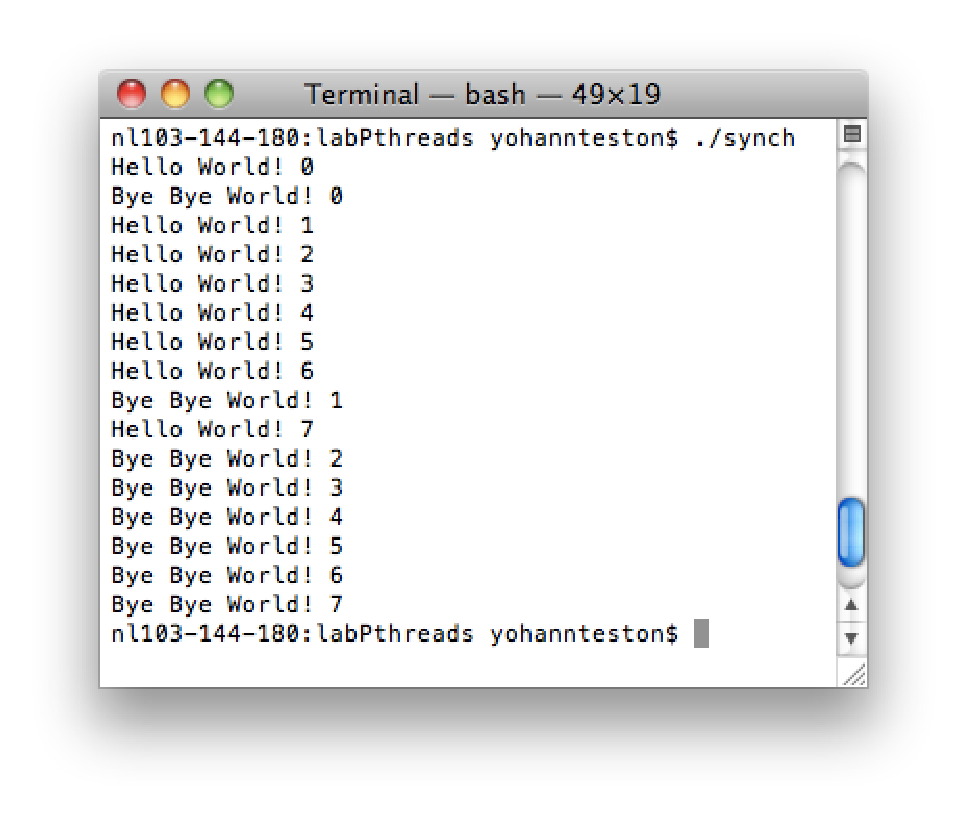
\includegraphics[width=\textwidth]{pic/q5.eps}
\end{center}


In \textit{spinwait.c}, the problem arises because the program does not load $state$'s value in a register for each test but do that once before the loop. So, when the last thread modifies $state$, its new value is not read by the other processes. Therefore, they keep spinning indefinitely. To avoid this, we have to make sure the compiler will generate a memory access each time $state$ is accessed. We can do that using the keyword $volatile$. We can then try again the program and see that everything works fine. 
